\chapter{Quantum Key Distribution}
Il Quantum Key Distribution (QKD) è un metodo di comunicazione sicuro che implementa un protocollo crittografico che coinvolge componenti di meccanica quantistica. Consente a due parti di produrre una chiave segreta casuale condivisa nota solo a loro, che può quindi essere utilizzata per criptare e decriptare i messaggi. Inoltre, invece di generare chiavi segrete una tantum utilizzate per più sessioni di comunicazione, i protocolli QKD possono fornire un flusso continuo di nuove chiavi segrete al fine di applicare la tecnica One Time Pad (OTP), la quale richiede che la chiave segreta non venga mai riutilizzata (venga utilizzata al massimo una volta).\\
Una proprietà importante e unica di questa tecnologia è il fatto che i due utenti in comunicazione possano rilevare la presenza di terze parti che cercano di acquisire informazioni sulla chiave. Ciò è reso possibile da una caratteristica fondamentale della meccanica quantistica: il processo di misurazione di un sistema quantistico, in generale, \textbf{disturba il sistema}. Una terza parte che cerca di intercettare la chiave deve in qualche modo misurarla, introducendo così anomalie rilevabili. Utilizzando sovrapposizioni quantistiche o l'\textbf{entanglement} quantistico e trasmettendo informazioni in stati quantistici, è possibile implementare un sistema di comunicazione che rilevi le intercettazioni. Se il livello di intercettazione è inferiore a una certa soglia, è possibile produrre una chiave di cui è garantita la sicurezza (ovvero, l'intercettatore non ha informazioni a riguardo), altrimenti non è possibile ottenere alcuna chiave sicura e la comunicazione viene interrotta.\\
Il protocollo QKD viene utilizzato solo per produrre e distribuire una chiave, non per trasmettere i dati del messaggio. Questa chiave può quindi essere utilizzata con qualsiasi algoritmo di crittografia scelto per criptare (e decriptare) un messaggio, che può quindi essere trasmesso su un canale di comunicazione standard \cite{shannon_communication_1949}.\\
La comunicazione quantistica implica la codifica delle informazioni in stati quantistici, o \textbf{qubit}, in contrasto con l'uso dei bit nella comunicazione classica. Di solito, i \textbf{fotoni} sono usati per rappresentare questi stati quantistici. Il QKD sfrutta alcune proprietà di questi stati quantistici per garantirne la sicurezza.\newpage
\noindent Esistono diversi approcci alla distribuzione delle chiavi quantistiche, ma possono essere divisi in due categorie principali a seconda della proprietà che sfruttano:
\begin{itemize}
    \item \textbf{Protocolli basati sulla preparazione e misurazione (PM):} Contrariamente alla fisica classica, l'atto della misurazione è parte integrante della meccanica quantistica. In generale, misurare uno stato quantistico sconosciuto cambia lo stato, in qualche modo. Questa è una conseguenza dell'indeterminatezza quantistica e può essere sfruttata per rilevare eventuali intercettazioni di comunicazione (che implicano necessariamente la misurazione) e, soprattutto, per calcolare la quantità di informazioni che è stata intercettata (es. protocolli BB84, B92).
    \item \textbf{Protocolli basati sull'entanglement (EB):} Gli stati quantistici di due (o più) oggetti separati possono essere "collegati" tra loro in modo tale da poter essere descritti da uno stato quantistico combinato, non come singoli oggetti. Questo è noto come \textbf{entanglement} e significa che, ad esempio, l'esecuzione di una misurazione su un oggetto influisce sull'altro. Se una coppia di oggetti quantistici collegati tra loro è condivisa tra due parti, chiunque intercetta uno dei due oggetti altera il sistema generale, rivelando la presenza della terza parte (e la quantità di informazioni che ha acquisito) (es. protocollo E91).
\end{itemize}

\noindent Come accennato in precedenza, i protocolli QKD non vengono utilizzati per crittografare i messaggi, ma vengono utilizzati per stabilire le chiavi segrete, che vengono poi utilizzate per criptare i messaggi. I messaggi crittografati vengono trasmessi attraverso i classici canali di comunicazione, cablati o wireless. Oltre al canale classico, i protocolli QKD richiedono un canale di comunicazione quantistico aggiuntivo per trasmettere gli stati quantistici che permettono poi di ricavare le chiavi segrete. Attualmente, il canale quantistico consiste in un canale a fibra ottica o wireless (aria).

\begin{figure}[H]
    \centering
    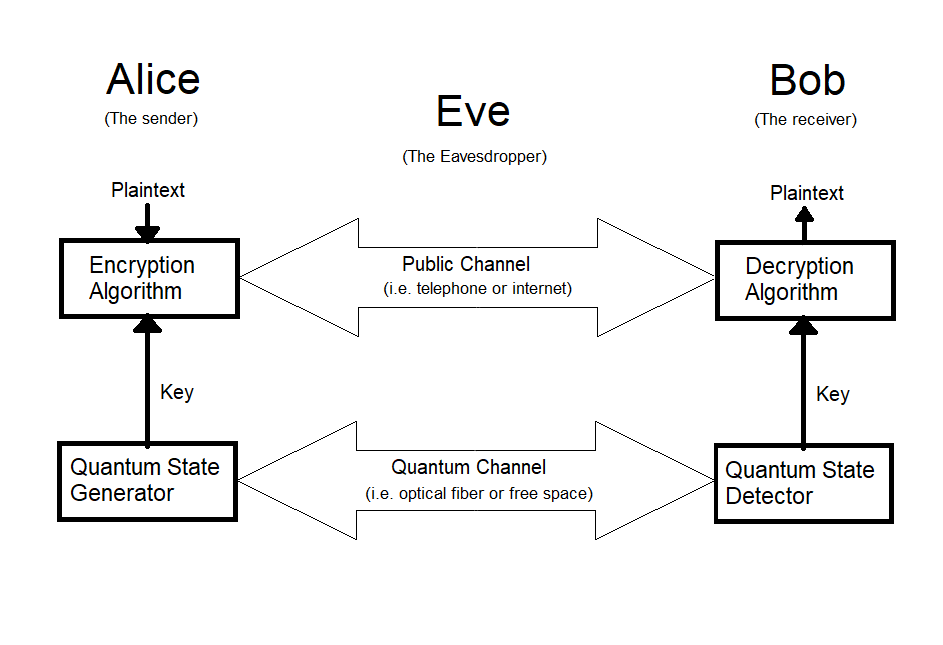
\includegraphics[width=0.85\textwidth]{MainContent/img/cap3/schema_QKD.png}
    \caption{QKD scheme}
    \label{fig:QKDscheme}
\end{figure}
\noindent
Come illustrato in Fig. \ref{fig:QKDscheme}, i protocolli QKD sono progettati per stabilire una chiave segreta solo tra una coppia di nodi mittente e destinatario, che sono collegati direttamente attraverso un canale quantistico senza alcun nodo intermedio. In quanto tali, sono protocolli peer-to-peer o point-to-point, sebbene il canale classico tra mittente e destinatario potrebbe non essere un collegamento diretto. Il canale classico viene utilizzato per trasmettere informazioni classiche, come il codice binario 1 o 0. D'altra parte, il canale quantistico viene utilizzato per trasmettere lo stato quantistico di una o più particelle (fotoni) \cite{yin_security_2016}.
Un’altra importante caratteristica operativa della QKD, quando viene utilizzata in sequenza per produrre chiavi di cifratura successive, come vedremo in seguito è la proprietà chiamata “forward-secrecy” delle chiavi: le chiavi successivamente scambiate con QKD sono indipendenti l’una dall’altra. Pertanto, la potenziale compromissione di una di esse non può portare alla compromissione delle altre. Questa è una caratteristica particolarmente apprezzabile sia per le reti ad elevata sicurezza, che per la memorizzazione a lungo termine dei dati (everlasting security).
Di seguito verrano descritti alcuni dei protocolli più noti, tra cui BB84, B92 e E91.
\newpage
\section{Protocollo BB84}
Questo protocollo, noto come BB84, prende il nome dai suoi inventori e dell'anno di pubblicazione \cite{bennett_quantum_2014}. Il mittente (tradizionalmente indicato come Alice) e il ricevitore (Bob) sono collegati da un canale di comunicazione quantistico che consente la trasmissione di stati quantistici. Nel caso dei fotoni, questo canale è generalmente una fibra ottica o semplicemente uno spazio libero. Inoltre, i due soggetti, comunicano tramite un canale pubblico classico, ad esempio tramite Internet. Il protocollo è progettato partendo dal presupposto che un attaccante (intercettatore denominato Eve) possa interferire in qualsiasi modo con il canale quantistico, mentre il canale classico deve essere autenticato e sicuro.\\
La sicurezza del protocollo deriva dalla codifica delle informazioni in stati non ortogonali. L'indeterminazione quantistica è causata dal fatto che questi stati non possono in generale essere misurati senza disturbare lo stato originale (Teorema di non clonazione). BB84 utilizza due coppie di stati, ciascuna coppia è coniugata all'altra e i due stati all'interno di una coppia sono ortogonali tra loro. Le coppie di stati di polarizzazione comunemente utilizzate sono:
\begin{itemize}
    \item La base rettilinea: verticale (0°) e orizzontale (90°)
    \item La base diagonale: 45° e 135°
\end{itemize}

Il primo passo è la trasmissione dei fotoni, Alice crea un bit casuale (0 o 1) e seleziona casualmente una delle sue due basi (rettangolare o diagonale). In seguito prepara uno stato di polarizzazione del fotone a seconda sia del valore del bit che della base, come mostrato nella Tabella \ref{tab:codifica_bit}. Quindi, ad esempio, uno 0 è codificato in base rettilinea (+) come stato di polarizzazione verticale e un 1 è codificato in base diagonale (x) come stato di 135°. Alice trasmette a Bob un singolo fotone nello stato predeterminato utilizzando il canale quantistico. Questo processo viene quindi ripetuto per ogni bit che Alice vuole inviare, registrando lo stato, la base e il tempo di trasmissione di ogni fotone.

\begin{table}[H]
\centering
    \begin{tabular}{|c|c|c|}
    \hline
    Basis & 0 & 1\\
    \hline
    $+$ & $\uparrow$ & $\rightarrow$\\
    \hline
    $\times$ & $\nearrow$ & $\searrow$\\
    \hline
    \end{tabular}
    \caption{Esempio di codifica dei Bit}
    \label{tab:codifica_bit}
\end{table}
\noindent Secondo la meccanica quantistica (in particolare l'indeterminazione quantistica), non è possibile ottenere i 4 stati di polarizzazione con un'unica misura, in quanto non sono tutti ortogonali. L'unica misura possibile è tra due stati ortogonali qualsiasi. Quindi, ad esempio, la misurazione con base rettilinea fornisce un risultato orizzontale o verticale. Se il fotone è stato creato come orizzontale o verticale (con base rettilinea), la misurazione fornirà lo stato corretto, ma se è stato creato con angolazione di 45° o 135° (con base diagonale), la misurazione con base rettilinea fornisce invece uno stato orizzontale o verticale a caso (con probabilità del 50\%). Inoltre, dopo questa misurazione il fotone è polarizzato nello stato in cui è stato misurato (orizzontale o verticale), e tutte le informazioni sulla sua polarizzazione precedente vengono perse.\\
Poiché Bob non conosce la base con cui sono stati codificati i fotoni, tutto ciò che può fare è selezionare una base a caso con cui misurare, rettilinea o diagonale. Questo viene fatto per ogni fotone che Bob riceve, registrando il tempo, la base di misurazione utilizzata e il risultato della misurazione. Dopo che Bob ha misurato tutti i fotoni, comunica con Alice tramite il canale pubblico classico. Alice trasmette le basi con cui sono stati polarizzati i fotoni inviati e Bob le basi con cui ognuno è stato misurato. Entrambi scartano le misurazioni dei fotoni (bit) in cui Bob ha utilizzato una base diversa da Alice e quelli restanti, misurati con la medesima base (quindi corretti), vengono utilizzati come chiave condivisa. Ecco un esempio in Fig. \ref{tab:BB84}:
\setlength\doublerulesep{0.3cm} 
\begin{table}[H]
\centering
    \begin{tabular}{|c|c|c|c|c|c|c|c|c|}
    \hline
    Bit randomici trasmessi da Alice & 0 & 1 & 1 & 0 & 1 & 0 & 0 & 1\\
    \hline \hline
    Basi utilizzate da Alice & $+$ & $+$ & $\times$ & $+$ & $\times$ & $\times$ & $\times$ & $+$\\
    \hline
    Polarizzazione fotoni inviati da Alice & $\uparrow$ & $\rightarrow$ & $\searrow$ & $\uparrow$ & $\searrow$ & $\nearrow$ & $\nearrow$ & $\rightarrow$\\
    \hline \hline
    Basi utilizzate da Bob per la misurazione & $+$ & $\times$ & $\times$ & $\times$ & $+$ & $\times$ & $+$ & $+$\\
    \hline
    Polarizzazione fotoni misurati da Bob & $\uparrow$ & $\nearrow$ & $\searrow$ & $\nearrow$ & $\rightarrow$ & $\nearrow$ & $\rightarrow$ & $\rightarrow$\\
    \hline \hline
    \multicolumn{9}{|c|}{Condivisione delle basi utilizzate tra Alice e Bob}\\
    \hline \hline 
    Chiave segreta condivisa & 0 & - & 1 & - & - & 0 & - & 1 \\
    \hline 
    \end{tabular}
    \caption{Esempio di funzionamento del protocollo BB84}
    \label{tab:BB84}
\end{table}
\newpage
\section{Protocollo B92}
Il protocollo B92 è una versione modificata del protocollo BB84 con la differenza fondamentale che, mentre il protocollo BB84 utilizza quattro diversi stati di polarizzazione del fotone (V=90°,H=0°,+45°,-45°), nel protocollo B92 ne vengono presi in considerazione solo due (uno dalla base rettilinea, convenzionalmente stato di polarizzazione H = 0° e uno da la base diagonale, convenzionalmente +45°). Il protocollo B92 può essere riassunto nei seguenti passaggi:
\begin{itemize}
    \item Alice invia una stringa di fotoni nello stato di polarizzazione H=0° o nello stato di polarizzazione +45°, scelti casualmente. Lo stato H corrisponderà al bit '0' mentre lo stato +45° corrisponderà al bit '1'.
    
    \begin{table}[H]
    \centering
        \begin{tabular}{|c|c|c|}
        \hline
        0 & 1\\
        \hline
        $\rightarrow$ & $\nearrow$\\
        \hline
        \end{tabular}
        \caption{Esempio di codifica dei Bit E92}
        \label{tab:codifica_bit_E92}
    \end{table}
    
    \item Bob sceglie casualmente tra base rettilinea e diagonale, per misurare la polarizzazione del fotone ricevuto.
    Se Bob misura con base rettilinea, ci sono due possibili casi: 
    \begin{enumerate}
        \item se il fotone incidente è polarizzato H, il risultato della misurazione sarà lo stato H con probabilità 100\%.
        \item se il fotone incidente è polarizzato +45°, allora il il risultato della misurazione sarà lo stato H o lo stato V con probabilità 50\%.
    \end{enumerate}   
    Pertanto, se il risultato della misurazione è lo stato V=90°, Bob può dedurre con sicurezza che lo stato di polarizzazione del fotone è +45°.
    
    Lo stesso ragionamento può essere effettuato in quest'altra situazione, in cui la misurazione -45° indicherà che lo stato di polarizzazione incidente del fotone è H.
    
    \item Dopo la trasmissione della stringa di fotoni, Bob annuncia i casi in cui il risultato della misurazione è stato "V" o "-45°" e il resto viene scartato da entrambi. Questi risultati possono essere utilizzati per generare una stringa di bit casuale tra Alice e Bob.
    
    \item Per la verifica delle intercettazioni, Bob e Alice condividono pubblicamente una parte della stringa di bit casuale generata e se il tasso di errore di bit supera un limite tollerabile, la chiave viene eliminata. In caso contrario, le due parti sono state in grado di generare una chiave sicura e simmetrica tra di loro.
\end{itemize}
\newpage
\section{Protocollo E91}
Il protocollo E91 utilizza coppie di fotoni "connessi" (entangled photons). Questi possono essere creati da Alice, da Bob o da un ente terzo. I fotoni vengono poi distribuiti in modo che Alice e Bob possiedano un fotone di ciascuna coppia. Il protocollo si basa su due proprietà dell' entanglement quantistico:
\begin{enumerate}
    \item Gli stati cosiddetti "intrecciati" sono perfettamente correlati nel senso che se Alice e Bob misurassero le particelle polarizzazioni verticali o orizzontali, otterrebbero sempre la stessa risposta con una probabilità del 100\%. Tuttavia, i risultati sono completamente casuali; è impossibile per Alice prevedere se lei (e quindi Bob) otterrà una polarizzazione verticale o una polarizzazione orizzontale. 
    \item Qualsiasi tentativo di intercettazione da parte di Eve distruggerebbe queste correlazioni e le due parti se ne accorgerebbero.
\end{enumerate}
In questo protocollo Alice misura ogni fotone che riceve utilizzando alcune basi tra $Z_0$, $Z_{\pi/8}$ e $Z_{\pi/4}$ mentre Bob sceglie le basi tra $Z_0$, $Z_{\pi/8}$ e $-Z_{\pi/8}$ dove $Z_{\theta}$ è la base $\{|\uparrow\rangle$ , $|\rightarrow\rangle\}$ ruotata di $\theta$. 
In seguito vengono formati due gruppi di fotoni: il primo è costituito da fotoni misurati utilizzando la stessa base da Alice e Bob, mentre il secondo contiene tutti gli altri fotoni. Per rilevare eventuali intercettazioni, i due possono calcolare un valore statistico $S$ utilizzando i coefficienti di correlazione tra le basi scelte dai due soggetti, come mostrato negli esperimenti di \textbf{Bell} \cite{noauthor_bell_2022}. Se i fotoni saranno ancora "intecciati" tra loro, risulterà $|S| = 2\sqrt{2}$. Se così non fosse, allora Alice e Bob possono concludere che Eve ha introdotto del disturbo nel sistema intercettando dei fotoni. Se il protocollo ha esito positivo, il primo gruppo può essere utilizzato per generare chiavi poiché quei fotoni sono completamente correlati (anti-allineati) tra Alice e Bob.

\newpage
\section{Attacchi ai protocolli di QKD}
\subsection{Intercettazione}
Il tipo più semplice di attacco possibile è l'attacco di intercettazione e re-invio, in cui Eve misura gli stati dei fotoni inviati da Alice e li invia nuovamente a Bob. Nel protocollo BB84, questo attacco produce errori nella trasmissione della chiave tra Alice e Bob. Poiché Eve non ha alcuna conoscenza della base in cui è codificato uno stato inviato da Alice, può solo cercare di indovinare in quale base misurare, allo stesso modo di Bob. Nel caso in cui scegliesse correttamente, misurerebbe lo stato di polarizzazione del fotone corretto inviato da Alice e invierebbe nuovamente lo stato corretto a Bob. Tuttavia, se scegliesse in modo errato, lo stato che misurerebbe sarebbe casuale e lo stato inviato a Bob sarebbe diverso dallo stato inviato da Alice. Se Bob poi misurasse questo stato con la stessa base inviata da Alice, anche lui otterrebbe un risultato casuale, con una probabilità del 50\%. La Tab. \ref{tab:BB84attack} mostra un esempio di questo tipo di attacco.

\setlength\doublerulesep{0.3cm} 
\begin{table}[H]
\centering
    \begin{tabular}{|c|c|c|c|c|c|c|c|c|}
    \hline
    Bit randomici trasmessi da Alice & 0 & 1 & 1 & 0 & 1 & 0 & 0 & 1\\
    \hline \hline
    Basi utilizzate da Alice & $+$ & $+$ & $\times$ & $+$ & $\times$ & $\times$ & $\times$ & $+$\\
    \hline
    Polarizzazione fotoni inviati da Alice & $\uparrow$ & $\rightarrow$ & $\searrow$ & $\uparrow$ & $\searrow$ & $\nearrow$ & $\nearrow$ & $\rightarrow$\\
    \hline \hline
    Basi utilizzate da Eve per la misurazione & $+$ & $\times$ & $+$ & $+$ & $\times$ & $+$ & $\times$ & $+$\\
    \hline
    Polarizzazione fotoni misurati e inviati da Eve & $\uparrow$ & $\nearrow$ & $\rightarrow$ & $\uparrow$ & $\searrow$ & $\rightarrow$ & $\nearrow$ & $\rightarrow$\\
    \hline \hline
    Basi utilizzate da Bob per la misurazione & $+$ & $\times$ & $\times$ & $\times$ & $+$ & $\times$ & $+$ & $+$\\
    \hline
    Polarizzazione fotoni misurati da Bob & $\uparrow$ & $\nearrow$ & $\nearrow$ & $\searrow$ & $\rightarrow$ & $\nearrow$ & $\uparrow$ & $\rightarrow$\\
    \hline \hline
    \multicolumn{9}{|c|}{Condivisione delle basi utilizzate tra Alice e Bob}\\
    \hline \hline 
    Chiave segreta condivisa & 0 & - & 0 & - & - & 0 & - & 1 \\
    \hline 
    Errori (Y = corretto, N = errato) & Y & - & N & - & - & Y & - & Y \\
    \hline 
    \end{tabular}
    \caption{Esempio di attacco al protocollo BB84}
    \label{tab:BB84attack}
\end{table}

\noindent Per verificare la presenza di un attaccante (intercettatore), Alice e Bob confrontano un sottoinsieme predeterminato dei bit rimanenti. Se una terza parte (Eve) avesse ottenuto informazioni sulla polarizzazione dei fotoni, ciò introdurrebbe errori nelle misurazioni di Bob. In realtà, altre condizioni ambientali possono causare errori in modo simile. Se più di \textbf{p} bit differiscono, la chiave viene scartata ed il processo viene ripetuto, possibilmente con un canale quantistico diverso, poiché la sicurezza della chiave non può essere garantita.
La probabilità che Eve scelga la base "sbagliata" è del 50\% (supponendo che Alice scelga a caso), e se Bob misurasse questo fotone intercettato nella base inviata da Alice otterrebbe comunque un risultato casuale, cioè un risultato errato con una probabilità del 50\%. La probabilità che un fotone intercettato generi un errore nella chiave è quindi del: 50\% × 50\% = 25\%. \\
Se invece, Eve dovesse venire a conoscenza delle basi utilizzate da Alice, potrebbe intercettare e inviare a Bob i fotoni senza che nessuno se ne accorga, ottenendo così la chiave condivisa tra i due. È per questo motivo che il canale classico, in cui vengono condivise le basi di misurazione, deve essere sicuro ed autenticato.

\subsection{Man in the middle}
I protocolli di  QKD sono vulnerabili ad un attacco man-in-the-middle se utilizzati senza autenticazione, poiché nessun principio noto della meccanica quantistica permette di "riconoscere" la controparte. Come nel caso classico, Alice e Bob non possono autenticarsi a vicenda e stabilire una connessione sicura senza alcuni mezzi per verificare le identità reciproche (come un segreto condiviso iniziale). Se Alice e Bob inizialmente possiedono un segreto condiviso, possono utilizzare uno schema di autenticazione insieme ad un protocollo di QKD per espandere la chiave condivisa e utilizzare una piccola quantità della di essa per autenticarsi la sessione successiva.

\subsection{Trojan-horse attacks}
In questo attacco, un eventuale malintenzionato utilizza il canale ottico che collega Alice e Bob e spedisce ad Alice degli impulsi di luce contenenti fotoni. Ogni impulso raggiunge il dispositivo di codifica ed è codificato con la stessa base del fotone normalmente preparato da Alice e poi inviato a Bob. Tuttavia, alcuni dei fotoni vengono riflessi (retro-diffusione) e consentono di ricavare informazioni sulle basi utilizzate da Alice, compromettendo così
la sicurezza del sistema \cite{gisin_trojan_2006}.

\subsection{Photon number splitting attack}
Nel protocollo BB84, Alice invia informazioni quantistiche a Bob usando singoli fotoni. Nella pratica molte implementazioni utilizzano impulsi laser attenuati ad un livello molto basso per inviare gli stati quantistici. Questi impulsi contengono un numero molto piccolo di fotoni (ad esempio 0.3 fotoni per impulso) e ciò significa che la maggior parte degli impulsi in realtà non contiene fotoni (nessun impulso viene inviato), alcuni impulsi contengono 1 fotone (come nella descrizione teorica) e alcuni impulsi contengono 2 o più fotoni.\\
Nel caso in cui l'impulso contenga più di un fotone, un intercettatore potrebbe separare i fotoni "extra", memorizzarli in una memoria quantistica e trasmetterne solo uno a Bob. L'intercettatore potrebbe quindi ascoltare le basi comunicate da Alice ed in seguito misurare i suoi fotoni nella base corretta, con lo scopo di ottenere informazioni sulla chiave senza introdurre errori rilevabili \cite{grazioso_photon-number-splitting-attack_2013}.

\subsection{Altre considerazioni}
Se si presume che l'attaccante abbia risorse illimitate, ad esempio che sia in possesso di risorse classiche e quantistiche, il protocollo BB84 si è dimostrato sicuro contro qualsiasi minaccia solo se vengono rispettate alcune condizioni:
\begin{itemize}
    \item Una terza parte non deve essere in grado di accedere fisicamente ai dispositivi di codifica e decodifica delle due entità comunicanti.
    \item I generatori di numeri casuali utilizzati devono essere affidabili e veramente casuali (Quantum Random Number Generator) \cite{herrero-collantes_quantum_2017}
    \item Il canale di comunicazione deve essere autenticato utilizzando uno schema di autenticazione incondizionatamente sicuro
    \item Il messaggio deve essere criptato utilizzando uno schema One-Time-Pad \cite{horstmeyer_physical_2013}
\end{itemize}